
\chapter{无线信号调制识别以及深度学习理论}
\label{chap: mod_rec_deep_learning_theo}
\section{引言}
在动态频谱接入(Dynamic Spectrum Access,DSA)中,感知周围的发射终端,以避免无线干扰并优化频谱分配,是无线认知的重要组成部分。 广播无线电、卫星信号、4G无线信号、雷达用户以及附近其他潜在无线电干扰源等信号具有不同的调制形式和特征,识别和区分这些信号是通信系统最基本的步骤,因此,必须针对信号的调制方式进行判别和解调。本章主要讨论信号调制的基本概念以及深度学习的基本理论。

\section{调制识别}

\subsection{信道对调制信号的影响}
无线信道模型是对无线信道的抽象描述,它能很好地反映真实环境中的信号传输规律。
无线通信数据信息主要以电磁波为载体通过无线信道传输。 
由于无线信道的环境复杂多变,电波以不同的传输方式(直射,反射,散射等)到达接收点,使得接收到的信号与发射的信号不同。
因此,只有准确预测无线信号的无线传播特性,如路径损耗和相位延迟,才能为无线网络提供合理的设计,部署和管理策略。\par

信道效应具备不确定性,在通信系统中是不可逆的。
真实的通信系统在进行信号传输时会经历许多影响,这给恢复和表示原始信号带来了很大难度。
热噪声在接收器处产生相对平坦的高斯白噪声,其形成信号的底噪。
由于温度和半导体物理材料自身特性,发射器和接收器的特性可能产生波动,
从而引起振荡器偏移导致符号时序偏移,采样速率偏移,载波频率偏移和相位差等。
这些效应可能导致信道之间的时间移位,缩放,线性混合、旋转等效应,给信息传输稳定性带来不利影响。
最后,根据在接收机处发射信号的到达模式,信号经过实际信道可能会经历随机滤波,产生幅度,相位变化和多普勒频移。
这就是通常所说的多径衰落或频率选择性衰落,其主要发生在当信号的传播路线上出现建筑物、车辆等障碍物,
阻碍了信号的视距传播,造成信号在空间中的反射,发生时频特性的变化。\par

\subsection{信道建模}

无线信号的调制识别可以看作是一个N类的决策问题。其中,输入是一个接收信号的复时间序列。
也就是说,我们以离散时间步长对无线电信号的同相和正交分量进行采样,
获得原始信号的$2 \times N$的复数值向量。我们将接收信号用方程\eqref{sec:eqt2_1}表示:
\begin{equation}\label{sec:eqt2_1}
r(t) = s(t)*c + n(t)
\end{equation}
其中,调制信号$s(t)$的生成,通过将连续信号或离散时间序列信号调制到具有变化的频率、相位、振幅、或多个变换的正弦波上得到。
缩放因子$c$是指信号上的一些路径损耗或恒定增益项,$n(t)$是反映热噪声的加性高斯白噪声过程。
在工程应用领域,这个简化的表达式在基于专家特征的决策统计方法中被广泛使用。\par

然而,实际的信道环境却比较复杂。发射信号$s(t)$在传播过程中经历多个信道效应, 最后在接收端被接收为$r(t)$。
这些信道效应包括:时间延迟,尺度缩放,相位旋转,频率偏移,加性热噪声,信道脉冲响应,以及所有的随机时变过程等。 
这些效应对信号的作用可以近似表示成方程 \eqref{sec:eqt2_2}:
\begin{equation}\label{sec:eqt2_2}
r(t) = e^{j*n_{Lo}(t)} \int_{\tau=0}^{\tau_{0}} s(n_{Clk}(t-\tau))h(\tau) + n_{Add}(t)
\end{equation}
方程\eqref{sec:eqt2_2}考虑了许多对于模型来说很重要的现实世界的影响:
通过残留载波随机游走过程调制$n_{Lo}(t)$,通过残留时钟振荡器随机游走重采样$n_{Clk}$,
与时变的旋转非恒定幅度脉冲响应$h(t-∞)$卷积,以及加性噪声$n_{Add}(t)$(可能不是白噪声)。
每个都可能导致未知的时变误差。考虑到现实世界中存在的无线信道的影响时,会使我们的接收信号表示复杂化。\par

考虑到传播信道的复杂性,对专家特征提取并进行分类决策建模是很难的。
这通常会迫使我们简化假设,构建易于处理的如方程\eqref{sec:eqt2_1} 所描述的基本模型;
然而,基本模型很难刻画复杂的信道特征,这样就造成了算法性能的上限较低,鲁棒性较差。
在本文中,我们主要关注包括所有上述影响的模拟传播环境中的实测数据,利用数据反映信道本身的特征,
而不是从理论上的进行信道建模指纹特征提取等。\par

\section{神经网络概述}

\subsection{神经元概述}	
神经网络(Neural Networks,NN),是一种模仿人类大脑神经行为,进行分布式并行信息处理的算法数学模型,
它起源于Rosenblatt等人在1957年提出的感知器模型\cite{rosenblatt1958perceptron}。
以监督学习为例,假设我们有训练样本集$(x(^i), y(^i))$,
那么神经网络算法能够提供一种复杂且非线性的假设模型$h_{W,b}(x)$ ,它具有参数$W, b$,
可以以此参数来拟合我们的数据。图\ref{fig_2_1}即是“神经元”的图示:\par
\begin{figure}[htbp]
	\centering
	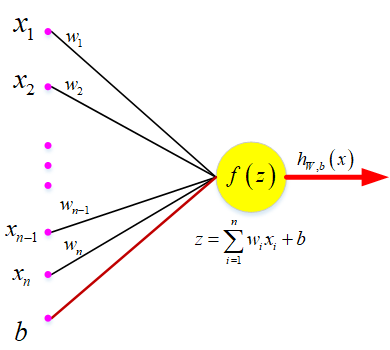
\includegraphics[scale=0.9]{figures/chapter_2/fig_2_1.png}\\
	\caption{神经元示意图}\label{fig_2_1}
\end{figure}
此“神经元”是一个以$x_1, x_2, ..., x_n$ 及截距$b$ 为输入值的运算单元,其输出为:
\begin{equation}
	h_{W,b}(x) = f(W^Tx) = f(\sum_{i=1}^n w_{i}x_i +b)
\end{equation} 
其中函数$f(z)$被称为“激活函数”,常用的激活函数有ReLU、Sigmoid、tanh等。在本论文中,激活函数$f(z))$选取可以降低``梯度消失``与``梯度爆炸``效应的ReLU函数\cite{glorot2011deep}\cite{krizhevsky2012imagenet}\cite{maas2013rectifier}:
\begin{equation}
	f(z) = 
	\begin{cases}
		1 & z <=0\\
		z & z > 0
	\end{cases}
\end{equation}
可以看出,ReLU激活函数在输入值小于零时输出为0,在大于0时为一条经过原点的直线,其相较于Sigmoid激活函数而言,具有如下优点:单侧抑制,具备较宽的兴奋边界,有利于梯度的传播并对网络引入稀疏性,缓和了梯度弥散问题,加快了网络的训练速度。\par
图\ref{sec:fig_2_2}和图\ref{sec:fig_2_3}分别是ReLU及Sigmoid的函数图像:
\begin{figure}[htbp]
	\centering
	\begin{minipage}[t]{0.48\textwidth}
		\centering
		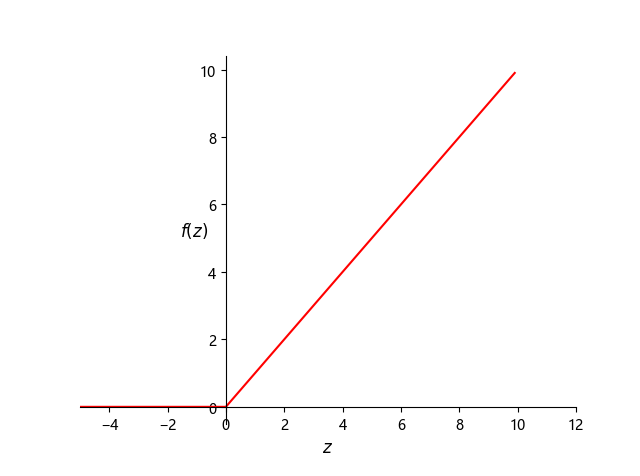
\includegraphics[width=8cm]{figures/chapter_2/fig_2_2.png}
		\caption{ReLU函数}\label{sec:fig_2_2}
	\end{minipage}
	\begin{minipage}[t]{0.48\textwidth}
		\centering
		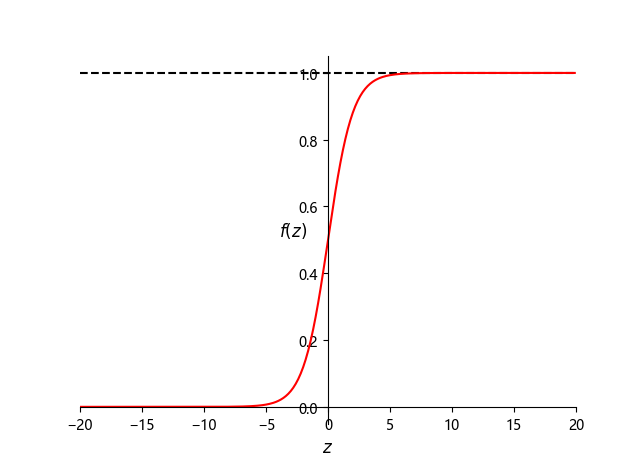
\includegraphics[width=8cm]{figures/chapter_2/fig_2_3.png}
		\caption{Sigmoid函数}\label{sec:fig_2_3}
	\end{minipage}
\end{figure}

\subsection{前馈神经网络}
前馈神经网络,是通过联结多个单一的“神经元”,使得一个“神经元”的输出作为另一个“神经元”输入的网络系统。图\ref{sec:fig_2_4}展示了一个简单的神经网络示意图。\par
\begin{figure}
	\centering
	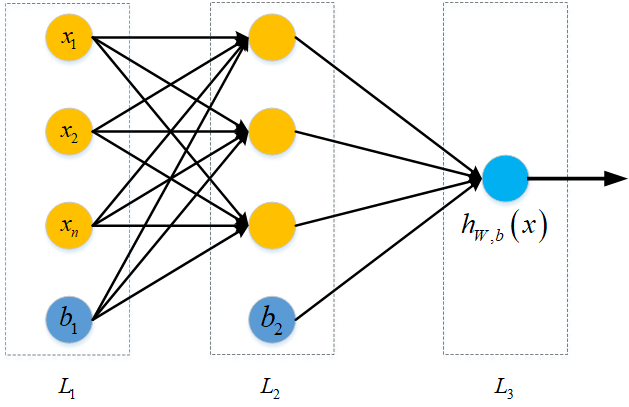
\includegraphics[scale=0.7]{figures/chapter_2/fig_2_4}\label{sec:fig_2_4}
	\caption{前馈神经网络}\label{sec:fig_2_4}
\end{figure}
假设用圆圈来表示神经网络的输入,偏置节点(截距项)就是标上“$b$”的圆圈。在神经网络中,最左边的一层作为输入层,输出层则是最右边的一层(本例采取只有一个节点的输出层)。中间层称为隐藏层,是由所有节点组成的。顾名思义,隐藏层就意味着它们的输出值无法在训练样本集中出现。并且,若不计算偏置单元,在该神经网络例子中,一共有$n(n=3)$个输入单元,$n(n=3)$个隐藏单元,以及一个输出单元。\par

 我们用$l_{*}$来表示网络的层数,本例中 ,我们将第$i$层记为$l_i$ ,于是$l_{0}$表示输入层,$l_L$表示输出层 。
利用$a^{(l)}_i$表示第$l$层第$i$单元的激活值(输出值)。当$l=1$时,$a^{(1)}_i = x_i$,即将输入值的第$i$个特征作为第$i$个输入值。对于给定参数集合$W,b$,利用所构建的神经网络的输出作为$h_{W,b}(x)$的结果。\par
 
第$l$层第$i$单元输入加权和(含偏置单元)用$z^{(l)}_i$表示。
上面的计算步骤叫作前向传播。
如果用$a^{(1)} = x$表示输入层的激活值,那么给定第$l$层的激活值$a^{(l)}$后,通过方程\eqref{eqt_2_10}的计算,可得第$l+1$层的激活值$a^{(l+1)}$。
\begin{align}
	\label{eqt_2_10}
	z^{(l+1)} &= W^{(l)} a^{(l)} + b^{(l)}=\sum_{j=l}^n W^{(l)}_{ij} x_j + b^{(l)}_i\\
	a^{(l+1)} &= f(z^{(l+1)})
\end{align}

线性代数对矩阵-向量的处理有一定的计算优势。将参数转为矩阵形式,然后利用这种优势精确并快速求解较复杂的神经网络。\par

上述讨论的是一种简单的、单隐层神经网络结构,接下来将构建另一种结构(神经元间的联接模式)更为复杂多样的神经网络,即包含多个隐层的深度神经网络。
最常见的一个例子是$n_l$层的神经网络,第$1$ 层是输入层,第$n_l$层是输出层,
中间的每个层$l$与层$l+1$紧密相联。这假如我们需要计算在该种模式下神经网络的输出结果,
根据前文描述的原理和网络层之间的等式关系,一步一步前向传播,从而得到第$L_2$层~第$L_{n_l}$ 层的激活值。
通过这种方式,我们需要的神经网络就构建成功。
同时,这种神经网络称为“前馈神经网络”,因为神经元之间没有形成闭环或者回路的连接。\par

\subsection{反向传播算法}
反向传播算法(Backpropagation,BP)是一种与最优化方法(如梯度下降法)结合使用的,用来训练人工神经网络的常见方法,最早由Rumelhart、Hiton等人正式提出\cite{rumelhart1986learning}。\par

假设我们有一个固定的样本集$\{ (x^{(1)}, y^{(1)})$, $\ldots$, $(x^{(m)}$, $y^{(m)}) \}$,它包含$m$个样本了,可以利用批量梯度下降算法就求解该网络。具体来说,对于单个样本$(x,y)$,我们假设其损失函数$J(W,b; x,y)$为方差代价函数,则有该样本的损失函数$J(W,b; x,y)$:
\begin{align}
	J(W,b; x,y) = \frac{1}{2} \left\| h_{W,b}(x) - y \right\|^2.
\end{align}
如果训练集包含$m$个样本,那么所有样本的整体损失函数$J(W,b)$为:
\begin{equation}
	\begin{aligned}
	J(W,b)
	&= \left[ \frac{1}{m} \sum_{i=1}^m J(W,b;x^{(i)},y^{(i)}) \right]
	+ \frac{\lambda}{2} \sum_{l=1}^{n_l-1} \; \sum_{i=1}^{s_l} \; \sum_{j=1}^{s_{l+1}} \left( W^{(l)}_{ji} \right)^2
	\\
	&= \left[ \frac{1}{m} \sum_{i=1}^m \left( \frac{1}{2} \left\| h_{W,b}(x^{(i)}) - y^{(i)} \right\|^2 \right) \right]
	+ \frac{\lambda}{2} \sum_{l=1}^{n_l-1} \; \sum_{i=1}^{s_l} \; \sum_{j=1}^{s_{l+1}} \left( W^{(l)}_{ji} \right)^2
	\end{aligned}
\end{equation}
上述定义中,第一项是均方差项,第二项是权重衰减项(即正则化项),
它的存在可以使过拟合以及权重绝对值均减小,
$\lambda$(即权重衰减系数)是这两项的平衡因子。
上述所介绍的代价函数在分类和回归问题中经常用到。
在二分类问题中,如果我们使用Sigmoid函数作为激活函数,由于Sigmoid激活函数的值域为$[0,1]$,
那么可以使用$y=0$或$y=1$,来代表两种类别的标签;
如果我们使用双曲正切激活函数$tanh$,那么可以选用$-1$和$+1$ 作为类别标签。\par

反向传播算法的思路如下:假设样例$(x,y)$,我们先通过“前向传播”的运算方法计算出网络中所有的激活值,其中包括$h_{W,b}(x)$的输出值。之后,针对第$l$层的每一个节点$i$,我们计算出其“残差”$\delta^{(l)}_i$,此残差表明了该节点对最终输出值的误差产生了多少影响。对于最终的输出节点,我们可以直接算出网络产生的激活值与实际值之间的差距,我们将这个差距定义为$\delta^{(n_l)}_i$(第$n_l$层表示输出层)。对于隐藏单元我们如何处理呢?我们将基于节点残差的加权平均值计算$\delta^{(l)}_i$,这些节点以$a^{(l)}_i$作为输入。以下几个步骤清楚地表述了反向传播算法:\par
进行前馈传导计算,利用前向传导公式,得到$L_2, L_3$, $\ldots$直到输出层$L_{n_l}$的激活值。
对输出层(第$n_l$层),计算:
\begin{align}
	\delta^{(n_l)}
	= - (y - a^{(n_l)}) \bullet f'(z^{(n_l)})
\end{align}
对于$l = n_l-1, n_l-2, n_l-3$, $\ldots$, $2$的各层,计算:
\begin{align}
	\delta^{(l)} = \left((W^{(l)})^T \delta^{(l+1)}\right) \bullet f'(z^{(l)})
\end{align}
计算最终需要的偏导数值:
\begin{align}
	\nabla_{W^{(l)}} J(W,b;x,y) &= \delta^{(l+1)} (a^{(l)})^T, \\
	\nabla_{b^{(l)}} J(W,b;x,y) &= \delta^{(l+1)}.
\end{align}
实现中应注意:在以上的第2步和第3步中,我们需要为每一个$i$值计算其$f'(z^{(l)}_i)$。前提是$f(z)$是sigmoid函数,同时$a^{(l)}_i$已经通过前向传导运算中得到。
最后,我们就梯度下降算法的使用进行较全面的总结。在下面的伪代码中,$\Delta W^{(l)}$是一个与矩阵$W^{(l)}$维度相同的矩阵,$\Delta b^{(l)}$是一个与$b^{(l)}$维度相同的向量。注意这里“$\Delta W^{(l)}$”是一个矩阵,而不是“$ \Delta$与$W^{(l)}$相乘”。批量梯度下降法中的一次迭代可以通过以下步骤完成:\par

对于所有$l$,令$\Delta W^{(l)} := 0$, $\Delta b^{(l)} := 0 $(设置为全零矩阵或全零向量)
对于$i(i \in \{1, 2, ..., m\})$,
使用反向传播算法计算$\nabla_{W^{(l)}} J(W,b;x,y)$和$\nabla_{b^{(l)}} J(W,b;x,y)$。
计算$\Delta W^{(l)} := \Delta W^{(l)} + \nabla_{W^{(l)}} J(W,b;x,y)$。
计算$\Delta b^{(l)} := \Delta b^{(l)} + \nabla_{b^{(l)}} J(W,b;x,y)$。
更新权重参数:
\begin{align}
	W^{(l)} &= W^{(l)} - \alpha \left[ \left(\frac{1}{m} \Delta W^{(l)} \right) + \lambda W^{(l)}\right] \\
	b^{(l)} &= b^{(l)} - \alpha \left[\frac{1}{m} \Delta b^{(l)}\right]
\end{align}
接下来,我们可以对梯度下降法算法不断迭代,减小损失函数$J(W,b)$的值,直到达到一定阈值或者终止条件,进而求解神经网络。

\section{卷积神经网络}
卷积神经网络(Convolutional Neural Network, CNN),是一种专门用来处理具有类似网格结构数据的神经网络,最早由LeCun在1989年提出\cite{lecun1989backpropagation}。
卷积神经网络至少在网络的某一层中使用卷积运算来替代一般的矩阵乘法运算,
在时间序列数据(可以认为是在时间轴上有规律地采样形成的一维网格)和图像数据(可以看作是二维的像素网格)等领域取得了较好的成果。。\par

\subsection{卷积运算}
\label{sec:the_convolution_operation}
卷积是一种对两个实变函数的线性运算,通常用星号表示:
\begin{equation}
s(t) = (x*w)(t) = \int x(\tau)w(t-\tau)d\tau
\end{equation}
在卷积网络的术语中,卷积的第一个参数(在这个例子中,函数$x$)通常叫做输入,第二个参数(函数$w$)叫核函数。
输出$ (x*w)$有时被称作特征映射。
如果我们假设$x$和$w$都定义在整数时刻$t$上,则卷积的离散形式:
\begin{equation}
s(t) = (x*w)(t) = \sum_{\tau = -\infty}^{\infty} x(\tau)w(t\tau).
\end{equation}
在机器学习应用中,输入通常是由样本的多维参数值组成的高维数组,而核通常是由优化算法对模型参数进行学习得到的多维数组。
通常我们称之为做张量。
因为在输入与核中的每一个元素都必须明确地分开存储,
所以通常情况下假设除了那些存储数值的有限点集以外的其他值都置为零。
这样,我们在实际操作中要想得到卷积中的无限求和,就可以通过求和有限个数组元素来实现。
在处理图像数据时,我们经常一次在多个维度上进行卷积运算。如果把一张二维的图像$I$作为输入,同时使用使用一个二维的核$K$,则有:
\begin{equation}
S(i,j) = (I*K)(i,j) = \sum_m \sum_n I(m,n) K(i-m, j-n).
\end{equation}
卷积是可交换的,我们可以等价地写作:
\begin{equation}
S(i, j) = (K*I)(i,j) = \sum_m \sum_n I(i-m, j-n) K(m, n).
\end{equation}
由于我们将核进行了翻转,所以出现了卷积运算的可交换性。从$m$增大的角度来看,输入的索引在增大,但是核的索引在减小。
我们将核翻转的唯一目的是实现可交换性。\par

\subsection{卷积特性}
(1) 卷积是一种无限强的先验\par
先验被认为是强或者弱取决于先验中概率密度的集中程度。
弱先验具有较高的熵值,例如方差很大的高斯分布。这样的先验允许数据对于参数的改变具有或多或少的自由性。
强先验具有较低的熵值,例如方差很小的高斯分布。这样的先验在决定参数最终取值时起着更加积极的作用。
一个无限强的先验需要对一些参数的概率置零并且完全禁止对这些参数赋值,无论数据对于这些参数的值给出了多大的支持。\par
我们可以把卷积网络类比成全连接网络,但对于这个全连接网络的权重有一个无限强的先验。
这个无限强的先验是说一个隐藏单元的权重必须和它邻居的权重相同,但可以在空间上移动。
这个先验也要求除了那些处在隐藏单元的小的空间连续的接受域内的权重以外,其余的权重都为零。\par
总之,我们可以把卷积的使用当作是对网络中一层的参数引入了一个无限强的先验概率分布。
这个先验说明了该层应该学得的函数只包含局部连接关系并且对平移具有等变性。\par

(2) 卷积性质\par
卷积运算通过三个重要的思想来帮助改进机器学习系统:稀疏交互、参数共享、等变表示。
传统的神经网络使用矩阵乘法来建立输入与输出的连接关系。
对于卷积,参数共享的特殊形式使得神经网络层具有对平移等变的性质。
如果一个函数满足输入改变,输出也以同样的方式改变这一性质,我们就说它是等变的。
特别地,如果函数$f(x)$与$g(x)$满足$f(g(x))= g(f(x))$,我们就说$f(x)$对于变换$g$具有等变性。
对于卷积来说,如果令$g$是输入的任意平移函数,那么卷积函数对于$g$具有等变性。
当处理时间序列数据时,这意味着通过卷积可以得到一个由输入中出现不同特征的时刻所组成的时间轴。
如果我们把输入中的一个事件向后延时,在输出中仍然会有完全相同的表示,只是时间延后了。
而这也正好对应到我们无线信号中的时移不变性。因此,我们可以很好的将\ref{con_net}应用到调制信号识别中。\par

(3) 卷积特征学习\par
一般而言,卷积神经网络的训练中最耗时的是特征学习。
通常输出层的计算代价相对不高,因为在通过若干层卷积池化之后,输入到该层的特征数量较小。
当使用梯度下降执行有监督训练时,每一次进行梯度计算需要完整地运行整个网络的前向传播和反向传播,
以使残差从输出层反馈到输入层。

利用那些无监督方式训练得到的特征是一种常用的减少卷积网络训练成本的方法。\par

通常,可以不通过监督训练而得到卷积核的基本策略主要有三类。
第一类是简单地随机初始化它们;
第二类是人工干预,比如设置卷积核的特定的方向和尺度来进行边缘检测;
最后,可以使用无监督的方法来学习卷积核。\par

使用无监督的标准来学习特征,我们可以认为是将CNN分成卷积层与分类层两部分,
网络允许我们将卷积层的特征参数确定与随后的分类层的参数学习相分离。
这样,便可以只需提取一次全部训练集的特征,作为随后分类层的新的训练集。
假设最后一层类似逻辑回归(Logistic Regression,LR)或者支持向量机,
那么分类层的学习通常是一种凸优化问题。\par
随机卷积核经常在卷积神经网络中表现得很好。
由Saxe的工作可知,如果我们对由卷积和随后的池化组成的层赋予随机权重,网络就会具备平移不变性和频率选择性\cite{saxe2011random}。
他们认为这提供了一种低时间成本的方法来选择卷积网络的结构:首先通过仅训练最后一层来评估几个卷积网络结构的性能,然后选择最好的结构并使用相对耗时的方法来训练整个网络。

这种选择卷积神经网络结构的方法,在作者看来时间成本相对较低:首先,通过单纯地训练最后一层的方式来评估几个卷积网络结构的性能;然后,比较这些网络结构并选取最优的网络,进行整个网络的训练。


\section{卷积自编码器}

自动编码器(autoencoder,AE)是一种无监督的学习算法,由Rumelhart在1986年第一次提出\cite{rumelhart1986learning}。
其优化目标是通过一些较低的中间隐层维度,使用均方误差(Mean Squared Error,MSE)等损失函数,最小化网络输出的重构误差。
它的目标是一种尽可能还原原始输入信号,主要用于数据的降维或者特征的提取。
为了还原输入信号,编码后的数据必须保留原始数据的主要特征。
如图\ref{sec:fig_2_5}所示,自编码器主要由两部分组成:
一个数据维度变换的编码器,以及一个生成重构信号的解码器 。
它内部还有一个隐藏层 ,可以产生原始数据编码后的低维表示,本质上都是对输入信号做某种非线性变换。\par
\begin{figure}[!h]
	\centering
	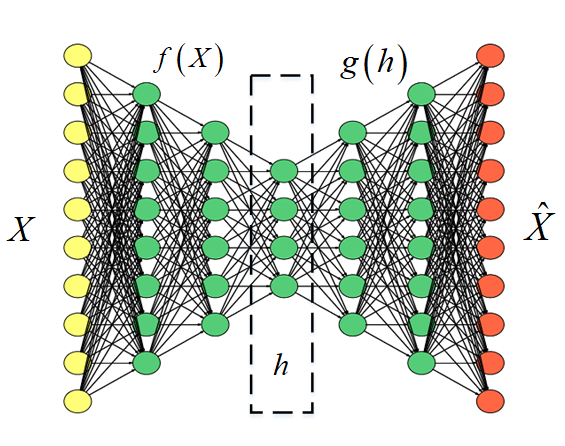
\includegraphics[scale=0.7]{figures/chapter_2/fig_2_5}
	\caption{自编码器}	\label{sec:fig_2_5}
\end{figure}

图\ref{sec:fig_2_5}中,将原始的训练数据集样本作为自编码器的输入,从输入层$X$到隐层$h$再到输出层$\hat{X}$的网络就是自编码器模型。
编码器将输入信号$X$变换成编码信号$h$,而解码器将编码信号$h$转换成输出信号$\hat{X}$。即:\par

\begin{equation}
	\begin{gathered}
		h=f(X)
		\\
		\hat{X}=g(h)=g(f(X))
	\end{gathered}
\end{equation}

通常,自编码器利用反向传播算法,将误差进行反向传播,并使用随机梯度下降算法等,以找到接近等式\eqref{sec:eqt2_3}中的最佳网络参数$\hat{\theta}$。
\begin{equation}\label{sec:eqt2_3}
	\hat{\theta} = \mathop{\arg\min}_{\theta} \sum(X − \hat{X})^2
\end{equation}

卷积自编码器(Convolutional Auto-Encode,CAE)是自编码器中的一种,主要是在编码器中加入了卷积层,
使得网络可以学习到数据的卷积相关特征。
编码器主要是由卷积层和池化层交叉组成的神经网络。
卷积的作用相当于一个滤波器,而池化则是提取不变特征。
CNN和CAE之间最主要的区别在于前者是进行有监督的卷积核学习,并且将提取的特征进行组合从而用来分类。
事实上,CNN通常被称为是一种监督学习;而CAE则通常被用来训练从输入数据中提取特征,从而重构输入数据。\par

CAE中的卷积层具有时移不变性以及受约束的参数搜索空间(相对于全连接层),因此非常适合于无线电时间序列信号表示。
我们使用dropout并在输入层加入噪声[7]对网络进行正则化,来增强模型的泛化能力。\par

\section{长短期记忆网络}

循环神经网络(Recurrent Neural Network)是一类用于处理序列数据的神经网络。
就像CNN主要是用于处理二维网格化数据的网络,RNN主要是用于处理时间序列$x^{(1)}, \dots, x^{(\tau)}$的神经网络。\par

长短期记忆网络(Long Short Term Network, LSTM)是一种被广泛应用的特殊 RNN 模型,可以学习数据的长期依赖信息。
它的网络结构如图\ref{sec:fig_2_6}所示。\par

\begin{figure}[!h]
	\centering
	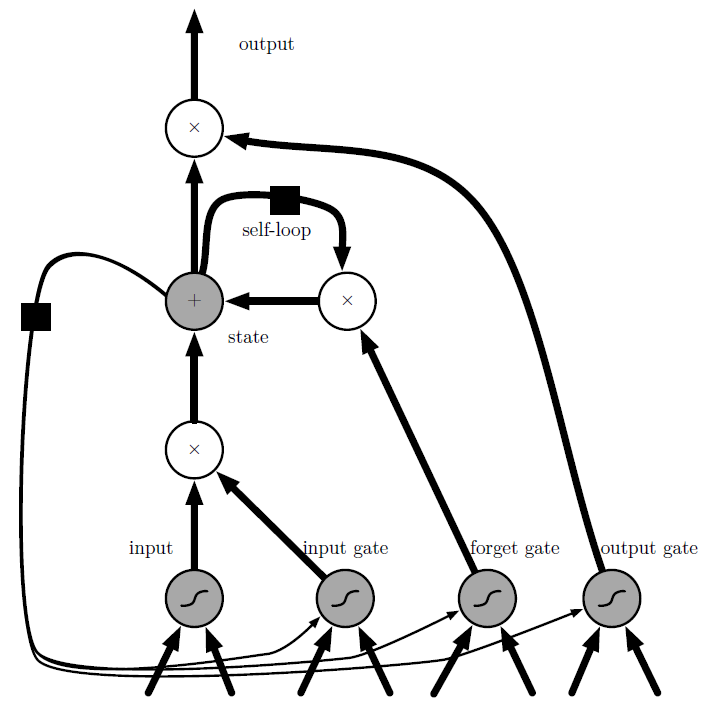
\includegraphics[scale=0.5]{figures/chapter_2/fig_2_6_1.png}
	\caption{LSTM网络结构框图}\label{sec:fig_2_6}
\end{figure}

LSTM 网络除了外部的RNN 循环外,还具有内部的“LSTM 细胞’’ 循环(自环),
因此LSTM 不是简单地向输入和循环单元的仿射变换之后施加一个逐元素的非线性。
与普通的循环网络类似,每个单元有相同的输入和输出,但也有更多的参数和控制信息流动的门控单元系统。

最重要的组成部分是状态单元$s_i^{(t)}$。
LSTM中包含自环,其权重(或相关联的时间常数)由遗忘门$f_i{(t)}$(forget gate)控制(时刻$t$和细胞$i$),
并由$sigmoid$单元将权重设置为0和1之间:\par
\begin{equation}
f_i^{(t)} = \sigma \Big( b_i^f + \sum_j U_{i,j}^f x_j^{(t)} + \sum_j W_{i,j}^f h_j^{(t-1)} \Big),
\end{equation}
其中$x^{(t)}$是当前输入向量,$h^{t}$是当前隐藏层向量,$h^{t}$包含所有~\glssymbol{LSTM}~细胞的输出。 
$b^f, U^f, W^f$分别是\gls{bias_aff}、输入权重和\gls{forget_gate}的循环权重。
因此LSTM细胞内部状态以如下方式更新,其中有一个条件的自环权重$f_i^{(t)}$:\par
\begin{equation}
	\begin{aligned}
		s_i^{(t)} = f_i^{(t)}  s_i^{(t-1)} +  g_i^{(t)}
		\sigma \Big( b_i + \sum_j U_{i,j} x_j^{(t)} + \sum_j W_{i,j} h_j^{(t-1)} \Big),
	\end{aligned}
\end{equation}

其中$b, U, W$分别是~\glssymbol{LSTM}~细胞中的\gls{bias_aff}、输入权重和\gls{forget_gate}的循环权重。
外部输入门(external input gate)单元$g_i^{(t)}$,以类似遗忘门(使用sigmoid获得一个0和1之间的值)的方式更新,
但其自身的参数:\par

\begin{equation}
	\begin{aligned}
	g_i^{(t)} = \sigma \Big( b_i^g + \sum_j U_{i,j}^g x_j^{(t)} + \sum_j W_{i,j}^g h_j^{(t-1)} \Big).
	\end{aligned}
\end{equation}

LSTM细胞的输出$h_i^{(t)}$也可以由输出门(output gate)~$q_i^{(t)}$关闭(使用sigmoid单元作为门控):\par
\begin{equation}
	\begin{gathered}
		h_i^{(t)} = \text{tanh}\big( s_i^{(t)} \big) q_i^{(t)}, \\
		q_i^{(t)} = \sigma \Big( b_i^o + \sum_j U_{i,j}^o x_j^{(t)} + \sum_j W_{i,j}^o h_j^{(t-1)} \Big),
	\end{gathered}
\end{equation}

其中$b^o, U^o, W^o$分别是\gls{bias_aff}、输入权重和\gls{forget_gate}的循环权重。
在这些变体中,可以选择使用细胞状态$s_i^{(t)}$作为额外的输入(及权重),输入到第$i$个单元的三个门,
如\ref{sec:fig_2_6}所示。
LSTM网络比简单的循环架构更易于学习长期依赖。

\section{神经网络优化算法}
在深度学习领域中,有很多现有的参数优化算法,
Ruder对常用的一阶和二阶、自适应与固定速率等学习算法进行了理论的阐述和比较\cite{ruder2016overview}。
在大多数机器学习问题中,我们主要关注任务的性能度量$P$,它是定义在测试集上对于模型性能的一个衡量标准。
但是,有时我们的性能P并不能达到,或者问题本身无解,这时,我们只是间接地优化$P$。
我们希望通过降低代价函数$J(\theta)$来提高$P$。
这一点与纯粹的优化不同,纯优化最小化目标 $J(\theta)$本身。
训练深度模型的优化算法通常也会包括一些针对机器学习目标函数的特定结构进行的优化。
即寻找神经网络上的一组参数$\theta$,它能显著地降低代价函数$J(\theta)$,
该代价函数通常包括整个训练集上的性能评估和额外的正则化项。

\subsection{统计梯度下降优化算法}
统计梯度下降(Stochastic Gradient Descent,SGD)及其变种
是机器学习尤其是深度学习中最常用的一种优化算法\cite{bottou2010large}。
它通过抽取数据的$m$个小批量(独立同分布的)样本,然后计算它们梯度均值,获得梯度的无偏估计。
算法\ref{alg:sgd}展示了SGD算法的迭代更新的方法。

\begin{algorithm}[ht]
	\caption{\gls{SGD}(\glssymbol{SGD})在第$k$个训练迭代的更新}
	\label{alg:sgd}
	\begin{algorithmic}
		\REQUIRE 学习速率 $\epsilon_k$
		\REQUIRE 初始参数$\theta$
		\WHILE{停止\gls{criterion}未满足}
		\STATE 从\gls{training_set}中采包含$m$个样本$\{ x^{(1)},\dots, x^{(m)}\}$ 的小批量,其中$x^{(i)}$对应目标为$y^{(i)}$
		\STATE 计算梯度估计: $\hat{g} \leftarrow + 
		\frac{1}{m} \nabla_{\theta} \sum_i L(f(x^{(i)};\theta),y^{(i)})$
		\STATE 应用更新:$\theta \leftarrow theta - \epsilon \hat{g}$
		\ENDWHILE
	\end{algorithmic}
\end{algorithm}

学习速率在SGD算法中是一个至关重要的参数。
之前,我们介绍的\,\glssymbol{SGD}\,使用固定的学习速率。
在实际应用中,有时随着学习的深入需要降低学习速率,
因此我们将第$k$步迭代的学习速率记作$\epsilon_k$。

这是因为\,\glssymbol{SGD}\,中梯度估计引入的噪声源($m$个训练样本的随机采样)并不会在\gls{minimum}处消失。
相比之下,当我们使用\gls{batch}\gls{GD}到达\gls{minimum}时,整个\gls{cost_function}的真实梯度会变得很小,
之后为$\mathbf{0}$,因此\gls{batch}\gls{GD}可以使用固定的学习速率。
保证\,\glssymbol{SGD}\,收敛的一个充分条件是
\begin{equation}
\label{eq:8.12}
	\begin{aligned}
		\sum_{k=1}^\infty \epsilon_k = \infty\\
		\sum_{k=1}^\infty \epsilon_k^2 < \infty
	\end{aligned}
\end{equation}
在实际应用中,一般会设置阈值$\tau$。学习速率将持续衰减,直到第$\tau$次迭代。
学习速率衰减的形式如公式\eqref{eqt_2_14}所示。
\begin{equation}
\label{eqt_2_14}
\epsilon_k = (1-\alpha) \epsilon_0 + \alpha \epsilon_\tau
\end{equation}
其中$\alpha = \frac{k}{\tau}$,表示衰减因子。
一般在$\tau$步迭代之后使$\epsilon$保持常数,使优化算法以较小的恒定速率学习模型参数。

\subsection{自适应矩估计优化算法}
\label{sec:adam}
自适应矩估计(Adaptive Moment Estimation,Adam),是一种自适应学习率的算法\cite{kingma2014adam}。
Adam基于低阶矩的自适应估计,是一种基于一阶梯度的随机目标函数优化算法。
该方法实施起来很简单,计算效率高,存储需求小,善于处理稀疏梯度,
并且非常适合于数据和参数较大时的参数优化,网络超参数通常不需要进行手动调整。
虽然有时学习速率需要手动修改默认值,但它对超参数的选择具有较强的鲁棒性。
Adam的整体流程如算法\ref{alg:adam}所示。
\begin{algorithm}[ht]
	\caption{Adam算法}
	\label{alg:adam}
	\begin{algorithmic}
		\REQUIRE 步长 $\epsilon$ (建议默认为: $0.001$)
		\REQUIRE 矩估计的指数衰减速率, $\rho_1$ 和 $\rho_2$ 在区间 $[0, 1)$内。
		(建议默认为:分别为$0.9$ 和 $0.999$)
		\REQUIRE 用于数值稳定的小常数 $\delta$  (建议默认为: $10^{-8}$)
		\REQUIRE 初始参数 $\theta$
		\STATE 初始化一阶和二阶矩变量 $s = 0 $, $r = 0$
		\STATE 初始化\gls{time_step} $t=0$ 
		\WHILE{没有达到停止\gls{criterion}}
		\STATE 从\gls{training_set}中采包含$m$个样本$\{ x^{(1)},\dots, x^{(m)}\}$ 的小批量,对应目标为$y^{(i)}$。
		\STATE 计算梯度:$g \leftarrow \frac{1}{m} \nabla_{\theta} \sum_i L(f(x^{(i)};\theta),y^{(i)})$ 
		\STATE $t \leftarrow t + 1$
		\STATE 更新有偏一阶矩估计: $s \leftarrow \rho_1 s + (1-\rho_1) g$
		\STATE 更新有偏二阶矩估计:$r \leftarrow \rho_2 r + (1-\rho_2)  g \odot g$
		\STATE 修正一阶矩的\gls{bias_sta}:$\hat{s} \leftarrow \frac{s}{1-\rho_1^t}$
		\STATE 修正二阶矩的\gls{bias_sta}:$\hat{r} \leftarrow \frac{r}{1-\rho_2^t}$
		\STATE 计算更新:$\Delta \theta = - \epsilon \frac{\hat{s}}{\sqrt{\hat{r}} + \delta}$ \ \  (逐元素应用操作)
		\STATE 应用更新:$\theta \leftarrow \theta + \Delta \theta$
		\ENDWHILE
	\end{algorithmic}
\end{algorithm}
在算法\ref{alg:adam}中,动量直接并入了梯度一阶矩(指数加权)的估计。
将动量加入RMSProp最直观的方法是将动量应用于缩放后的梯度。
其次,Adam包括偏置修正,修正从原点初始化的一阶矩(动量项)和(非中心的)二阶矩的估计。
\par

\subsection{RMSProp优化算法}
RMSprop是一个广泛应用的却未被发表的自适应学习率的算法,
该算法由Geoff Hinton在其Coursera课堂的课程6e中提出\cite{tieleman2012lecture}。
RMSProp将学习率分解成一个平方梯度的指数衰减的平均,利用衰减系数来控制历史信息的获取多少,以使其能够在找到凸碗状结构后快速收敛,适合处理非平稳目标。\par

RMSProp算法的标准形式如\ref{alg:rms_prop}所示。
\begin{algorithm}[ht]
	\caption{RMSProp算法}
	\label{alg:rms_prop}
	\begin{algorithmic}
		\REQUIRE 全局学习速率 $\epsilon$,衰减速率$\rho$
		\REQUIRE  初始参数$\theta$
		\REQUIRE 小常数$\delta$,通常设为$10^{-6}$(用于被小数除时的数值稳定)
		\STATE 初始化累积变量 $r = 0$
		\WHILE{没有达到停止\gls{criterion}}
		\STATE 从\gls{training_set}中采包含$m$个样本$\{ x^{(1)},\dots, x^{(m)}\}$ 的小批量,对应目标为$y^{(i)}$。
		\STATE 计算梯度:$g \leftarrow  
		\frac{1}{m} \nabla_{\theta} \sum_i L(f(x^{(i)};\theta),y^{(i)})$ 
		\STATE 累积平方梯度:$r \leftarrow \rho
		r + (1-\rho) g \odot g$
		\STATE 计算参数更新:$\Delta \theta =
		-\frac{\epsilon}{\sqrt{\delta + r}} \odot g$  \ \  ($\frac{1}{\sqrt{\delta + r}}$ 逐元素应用)
		\STATE 应用更新:$\theta \leftarrow \theta + \Delta \theta$
		\ENDWHILE
	\end{algorithmic}
\end{algorithm}

\subsection{选择正确的优化算法}
\label{sec:choosing_the_right_optimization_algorithms}
在本节中,我们讨论了一系列算法,通过自适应每个模型参数的学习速率以解决优化深度学习中的难题。
然而,对于哪一种优化算法具有最优的性能,目前仍没有确定。
Schaul等人对现有的一些神经网络优化算法在几个学习任务上进行了比较\cite{schaul2013unit}。
结果显示,一般情况下,自适应学习速率的算法(如以RMSProp和AdaDelta等)具备较强的鲁棒性;
在各个任务上,每种优化算法所取得的性能相近,没有某个确定的算法能绝对地优于其他算法。\par

目前,使用率较高的优化算法主要有SGD、包含动量项的SGD、基于动量的RMSProp、AdaDelta和Adam等。
此时,选择哪一个算法则主要取决于使用者的喜好以及对不同优化算法的熟悉程度(以便调节超参数)。
本文中,根据不同的条件,综合使用以上几种优化算法,以期能够达到性能的最优。

\section{本章小结}
本章对于论文中所用到的相关理论知识进行了较为系统的阐述,主要介绍了信号调制及深度学习的理论基础。
我们首先介绍了信道对于调制识别的影响,并基于数据利用网络自学习信道的影响,避免了直接对于信道建模的误差影响;
接下来,介绍了神经元、前馈神经网络、卷积神经网络、自编码器等深度学习的基本理论和基本网络架构;
最后,介绍了最近较为流行的几种神经网络优化算法,并分析了各种算法的理论基础。
